\section{Data}\label{sec:data}

\subsection{Conflict and unrest events}\label{sec:data-acled}

Event data come from the Armed Conflict Location \& Event Data Project
\citep[ACLED;][]{raleigh2010acled}. ACLED records the date, location, actors and type
of individual events of political violence and demonstrations, compiled from news
media, local partners and other sources. We use events from 1 January 2018 to
31 December 2024 and group ACLED event types into two outcomes:
\emph{violent conflict} (battles, explosions/remote violence and violence against
civilians) and \emph{social unrest} (riots and protests). Events are aggregated to a
regular $0.5^\circ \times 0.5^\circ$ longitude--latitude grid, the resolution of
PRIO-GRID \citep{tollefsen2012priogrid}, and to calendar weeks. For cell $s$ and week
$t$, let $N^{(j)}_{st}$ be the number of events of type $j$, and let
\[
Y_{st} = \mathbf{1}\Bigl\{\textstyle\sum_{j \in \mathcal{J}} N^{(j)}_{st} > 0\Bigr\},
\]
where $\mathcal{J}$ is the set of event types of the outcome being modelled. The two
outcomes are analysed separately.

The joint analysis covers two regions. The larger one, Africa and the Middle East, is
the box from $20^\circ$W to $65^\circ$E and from $36^\circ$S to $45^\circ$N (the AME
region) without the
European countries that its northern corner contains (Spain, Portugal, France, Italy,
Malta, Greece, the Balkans and the part of Russia in the box), together with the
French islands of Mayotte and R\'eunion. ACLED covers most of these countries only
from 2020, and their dense, well-reported protest with almost no armed conflict is
unlike the rest of the region. Turkey, the Caucasus, Iran, Central Asia and
Afghanistan remain. \todo{Number of countries (job 29 log).} The smaller region, West Africa and the Sahel, is described in
Section~\ref{sec:app-joint}.

Event weeks are rare. Figure~\ref{fig:data} shows where and when events are recorded
in the AME region, which has 12{,}995 cells. Over 2018--2024, 2.4\% of covered
cell-weeks in the region contain at least one conflict event and 1.8\% at least one
unrest event; over all covered cell-weeks worldwide the shares are 1.3\% and 2.1\%.
Events are concentrated in
space:
\begin{itemize}
\item a third of the cells in the region (34.0\% for conflict, 32.6\% for unrest)
record any event at all;
\item the 1\% of cells with the most event weeks account for 29\% of all conflict event
weeks and 32\% of all unrest event weeks;
\item fewer than 1\% of cells record events in more than half of all weeks. These
cells, for example in Syria, Yemen, northeastern Nigeria and eastern Democratic
Republic of the Congo, are one reason why recent history is such a strong predictor
(Section~\ref{sec:data-history}).
\end{itemize}
The two outcomes have different geographies. Conflict forms large contiguous regions:
the central Sahel and Lake Chad basin, the Sudans and Ethiopia, Somalia, eastern Congo,
Yemen and Syria--Iraq. Unrest is densest in North Africa,
Turkey, Iran, South Africa and the Great Lakes region, where population and media
coverage are high. The weekly share of cells with an event rises over the period. For
conflict it goes from about 2\% in 2018 to about 2.5\% in 2024, and for unrest from
about 1.2\% to between 2\% and 3\%. The test period is therefore not exchangeable with
the early training years. The series also has isolated weeks with far fewer events
than the neighbouring weeks. We checked whether they arise in our construction of the
table. No week is split between the partitions of the source table, every cell-week
appears once, and the number of cells is constant in the weeks around each of them.
The dips are therefore present in the weekly counts of the source partitions, and we
keep them as recorded. \todo{Sensitivity of the main results to excluding these
weeks.}

\begin{figure}
\centering
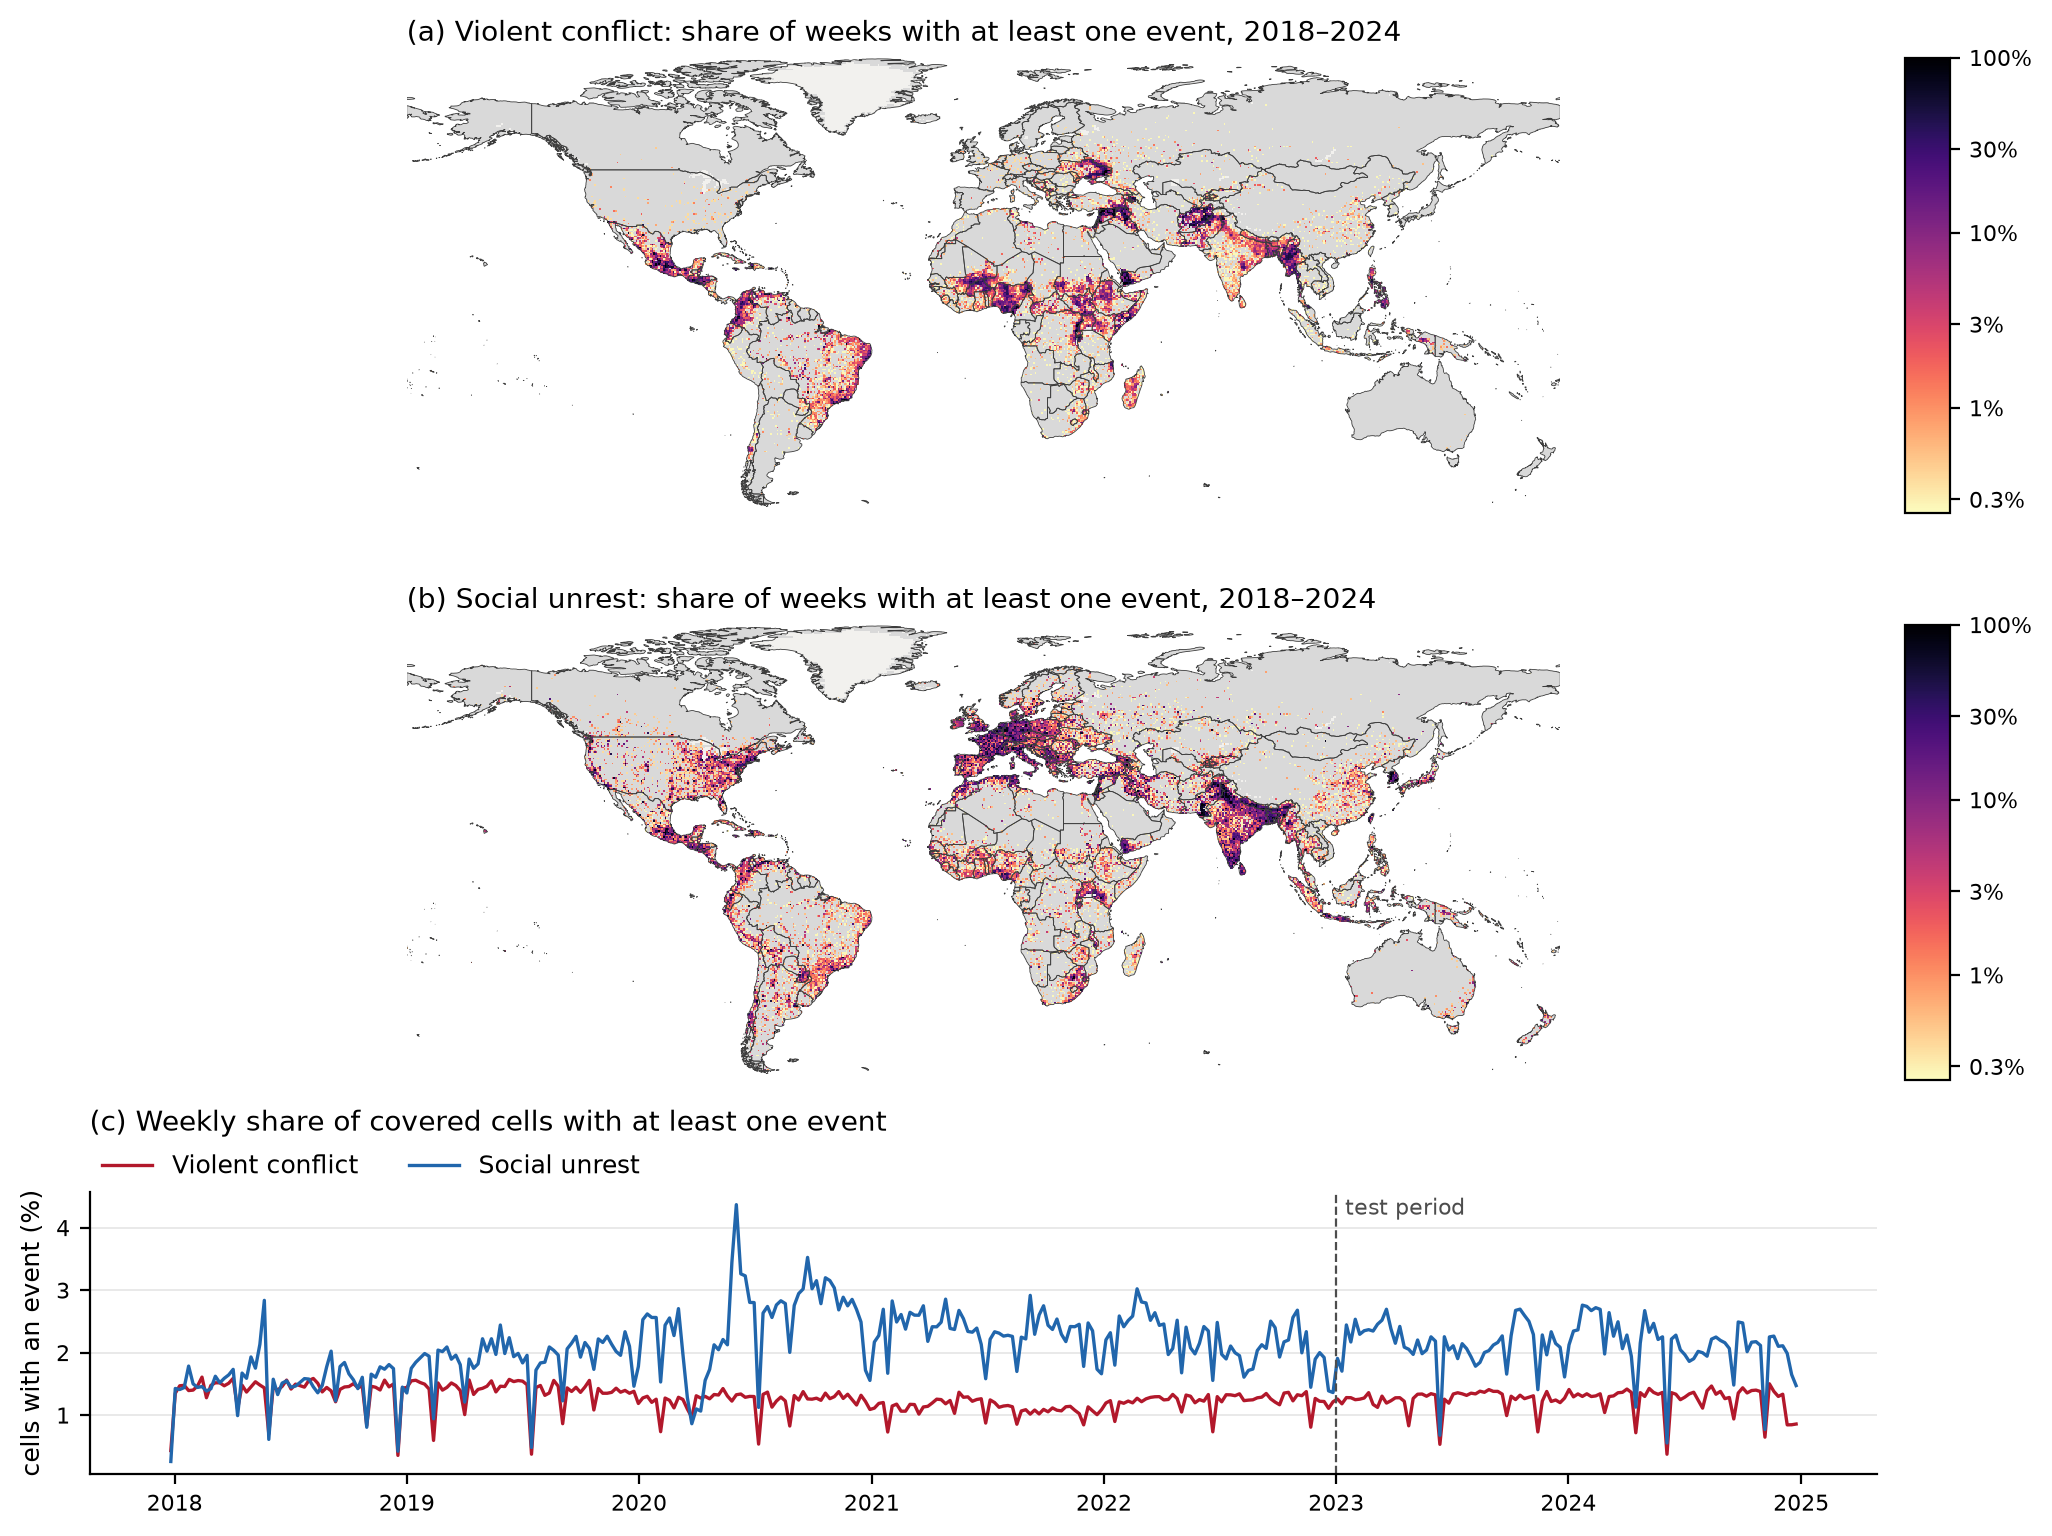
\includegraphics[width=\textwidth]{figures/data_events.png}
\caption{ACLED events on the $0.5^\circ$ grid in the AME region (Africa, the Middle
East and adjacent regions), 2018--2024, over covered cell-weeks. (a, b) Share of weeks with at least one event in
each cell, for violent conflict and social unrest (logarithmic colour scale); grey cells
have no event week. (c) Weekly share of covered cells in the region with at least one
event. The dashed line marks the start of the test period.}\label{fig:data}
\end{figure}

The grid consists of the $0.5^\circ$ cells that intersect a country, excluding cells
without a terrestrial biome. Cell-weeks in a country before its ACLED coverage start
are unobserved, not event free, and are removed. Since the probability that an event
is recorded depends on media and partner density, the outcome combines occurrence
and reporting \citep{weidmann2016closer}; the latent fields of
Section~\ref{sec:methods} absorb spatially smooth reporting differences together with
unmeasured drivers of risk, and we interpret them accordingly. The construction of the
table, including the repair of duplicated cell-weeks in the original pipeline, is
described in Section~\ref{supp:data-table} of the Supplementary Material.

\subsection{Recent event history}\label{sec:data-history}

For each cell and week we compute the number of events of each type in the four
preceding weeks, $L^{(j)}_{st} = \sum_{l=1}^{4} N^{(j)}_{s,t-l}$, using only past
weeks of the same cell. In the models of Section~\ref{sec:methods} the history enters
through $h_{st} = \log\bigl(1 + \sum_{j \in \mathcal{J}} L^{(j)}_{st}\bigr)$ for the
outcome being modelled, and through the corresponding quantity for the other outcome
as an additional covariate. Cell-weeks whose four-week history is incomplete, at the
start of the series and of each country's coverage, are dropped from the parametric
latent models. The boosting models, and the boosting offset of the hybrid models,
keep these rows and receive the incomplete history as missing.

\subsection{Environmental, socioeconomic and national covariates}\label{sec:data-cov}

Covariates are listed in Table~\ref{tab:covariates}. They vary at three
resolutions, which is central to the identification arguments of
Section~\ref{sec:methods-confounding}:
\begin{enumerate}
\item \emph{cell--week}: daily minimum and maximum temperature, heat index and
wet-bulb globe temperature (CHIRTS), precipitation (CHIRPS), PM$_{2.5}$ (CAMS) and a
drought index (Global Drought Observatory);
\item \emph{cell}: population (GHSL), river length and lake area (Natural Earth),
malaria risk (Malaria Atlas Project), terrestrial biome (RESOLVE Ecoregions) and,
in the boosting models only, an indicator of $|\mathrm{latitude}| < 30^\circ$;
\item \emph{country--year}: GDP per capita, access to electricity, the
Environmental Performance Index (EPI), the V-Dem liberal democracy index, and
per-capita greenhouse gas emissions, material footprint and ecological footprint.
\end{enumerate}
Food insecurity, the population in each IPC phase, is available for subnational
regions and periods and is apportioned to cells by population share.

Climate variables enter as their means over the four weeks before the current week,
as standardised anomalies with respect to a cell- and calendar-month-specific
climatology of the training years 2018--2022. Covariates are standardised with
training-period means; missing values are set to zero and a missingness indicator
enters for each national indicator and for IPC. Missingness is substantial (IPC phases
62.7\% of rows, PM$_{2.5}$ 55.5\%, GDP 3.6\%) and unlikely to be at random.
Section~\ref{supp:data-cov} of the Supplementary Material lists the covariates and
sources (Table~\ref{tab:covariates}) and details the anomalies and missing values.

